%
\documentclass[12pt]{article}

% The usual packages
\usepackage{fullpage}
\usepackage{breakcites}
\usepackage{setspace}
\usepackage{endnotes}
\usepackage{float}
\usepackage{amsmath}
\usepackage{amsfonts}
\usepackage{amssymb}
\usepackage{rotating}
\usepackage{dcolumn}
\usepackage{longtable}
\usepackage{microtype}
\usepackage{graphicx}
\usepackage{hyperref}
\usepackage[usenames,dvipsnames]{color}
\usepackage{url}
\usepackage{natbib}
\usepackage{framed}
\usepackage{lipsum}
\usepackage[font=small,labelfont=sc]{caption}
\restylefloat{table}
\bibpunct{(}{)}{;}{a}{}{,}

% Set paragraph spacing the way I like
\parskip=0pt
\parindent=20pt

% Define mathematical results
\newtheorem{lemma}{Lemma}
\newtheorem{proposition}{Proposition}
\newtheorem{theorem}{Theorem}
\newtheorem{claim}{Claim}
\newenvironment{proof}[1][Proof]{\begin{trivlist}
\item[\hskip \labelsep {\bfseries #1}]}{\end{trivlist}}
\newenvironment{definition}[1][Definition]{\begin{trivlist}
\item[\hskip \labelsep {\bfseries #1}]}{\end{trivlist}}
\newenvironment{example}[1][Example]{\begin{trivlist}
\item[\hskip \labelsep {\bfseries #1}]}{\end{trivlist}}
\newenvironment{remark}[1][Remark]{\begin{trivlist}
\item[\hskip \labelsep {\bfseries #1}]}{\end{trivlist}}

% Set up fonts the way I like
\usepackage{tgpagella}
\usepackage[T1]{fontenc}
%\usepackage[T1]{fontenc}
\usepackage[bitstream-charter]{mathdesign}

%% Set up lists the way I like
%Redefine the first level
\renewcommand{\theenumi}{\arabic{enumi}.}
\renewcommand{\labelenumi}{\theenumi}
%Redefine the second level
\renewcommand{\theenumii}{\alph{enumii}.}
\renewcommand{\labelenumii}{\theenumii}
%Redefine the third level
\renewcommand{\theenumiii}{\roman{enumiii}.}
\renewcommand{\labelenumiii}{\theenumiii}
%Redefine the fourth level
\renewcommand{\theenumiv}{\Alph{enumiv}.}
\renewcommand{\labelenumiv}{\theenumiv}

%% Setup the section headers the way I like
\usepackage{titlesec}
\titleformat{\section}
{\normalfont\large\bfseries\centering}{\thesection}{1em}{}
\titleformat{\subsection}
{\normalfont\normalsize\bfseries}{\thesubsection}{1em}{}

% Create footnote command so that my name
% has an asterisk rather than a one.
\long\def\symbolfootnote[#1]#2{\begingroup%
\def\thefootnote{\fnsymbol{footnote}}\footnote[#1]{#2}\endgroup}

\hypersetup{
 pdftitle={Arguing for a Negligible Effect}, % title
 pdfauthor={Carlisle Rainey}, % author
 pdfkeywords={hypothesis testing} {no effect} {negligible effect} {substantive significance},
 pdfnewwindow=true, % links in new window
 colorlinks=true, % false: boxed links; true: colored links
 linkcolor=Sepia, % color of internal links
 citecolor=Sepia, % color of links to bibliography
 filecolor=Sepia, % color of file links
 urlcolor=Sepia, % color of external links
 menucolor=Sepia
}
\usepackage[normalem]{ulem}

\begin{document}

%\maketitle
\begin{center}
{\LARGE Arguing for a Negligible Effect}\\\vspace{2mm}
\vspace{3mm}
Carlisle Rainey\symbolfootnote[1]{Carlisle Rainey is an Assistant Professor of Political Science, University at Buffalo, SUNY, 520 Park Hall, Buffalo, NY 14260 (\href{mailto:rcrainey@buffalo.edu}{rcrainey@buffalo.edu}). I thank Jason Barabas, Scott Clifford, Justin Esarey, Mark Fredrickson, Brad Gomez, Jennifer Jerit, Jonathan Nagler, Bob Jackson, Dave Siegel,  Deb Sinha, participants at the 2012 meeting of the Society for Political Methodology, and several anonymous reviewers for helpful comments on previous versions of this manuscript. I especially thank Yanna Krupnikov, William Clark, and Matt Golder for making their data available for me. Replication materials, supporting information, and updates can be obtained at \href{http://www.carlislerainey.com/research/arguing-for-a-negligible-effect/}{crain.co/nme}. Replication materials are also available at the AJPS Dataverse (\href{http://dvn.iq.harvard.edu/dvn/dv/ajps}{http://dvn.iq.harvard.edu/dvn/dv/ajps}).}\\\vspace{3mm}
Forthcoming in the \textit{American Journal of Political Science}.
\end{center}

%\singlespace
%\begin{center}
%Word Count: 5,636
%\end{center}\vspace{3mm}

\begin{quote}
\begin{center} Abstract\end{center}
Political scientists often theorize that an explanatory variable should have ``no effect''  and support this claim by demonstrating that its coefficient's estimate is not statistically significant. This empirical argument is quite weak, but I introduce applied researchers to simple, powerful tools that can strengthen their arguments for this hypothesis. With several supporting examples, I illustrate that researchers can use 90\% confidence intervals to argue against meaningful effects and provide persuasive evidence for their hypothesis.
\end{quote}

\doublespace


Political scientists often theorize that particular variables should not matter.\footnote{A growing literature in political science (e.g., \citealt{Bowers2012}) draws a distinction between inferences that focuses on unit-level treatment effects (i.e., a ``sharp null'') and average population treatment effects (i.e., a ``weak null''). For presentational purposes, I focus on hypotheses concerning average effects, but the key ideas hold regardless of one's conceptual approach (e.g., \citealt{RosenbaumSilber2009}).} \cite{Fearon1994} argues that (observable) military strength has no direct effect on bargaining once an international crisis begins. \cite{Svolik2008} suggests that economic development does not effect the timing of authoritarian reversals. \cite{FearonLaitin2003} contend that ethnic and religious diversity do not make civil wars more likely. \cite{KamPalmer2008} propose that education has no effect on political participation. These authors are not alone. On average, more than one article per issue of the \textit{American Political Science Review} and \textit{American Journal of Political Science} in 2011 and 2012 argues that some variable should have a negligible effect, at least in a particular context.\footnote{See the Supporting Information for the details of my review. Overall, I find that about one-third of the articles that present explicit hypotheses contain at least one hypothesis of a negligible effect. The Supporting Information also provides a brief summary of each article's theoretical argument for negligible effects.}
 
While political scientists commonly consider a lack of statistical significance as evidence for a negligible effect,  \cite{Westlake1979} points out that this is neither necessary nor sufficient evidence for the claim.\footnote{Under the standard two-tailed null hypothesis significance test, the research hypothesis posits that that effect is non-zero ($H_r : \Delta \neq 0$) and the null hypothesis posits that the effect is exactly zero ($H_0 : \Delta = 0$). If as or more extreme data would occur only rarely if the null hypothesis were correct, then the researcher rejects the null hypothesis in favor of the research hypothesis. If as or more extreme data would occur fairly often if the null hypothesis were correct, then the researcher fails to reject the null hypothesis.} As an alternative, I introduce the TOST approach \citep{BergerHsu1996}, which enables analysts to make more compelling arguments for their hypothesis of a negligible effect by explicitly testing whether meaningful effects are plausible.\footnote{Biostasticians typically refer to the problem of determining whether two parameters are similar as ``equivalence'' or ``bioequivalence.'' \cite{Wellek2010} provides an excellent overview of this literature. Biostatistians also draw a careful distinction between \textit{population} bioequivalence studies and \textit{individual} bioequivalence studies. I borrow heavily from the literature on population bioequivalence. See \cite{Anderson1993} for an excellent but accessible discussion of the differences between individual and population bioequivalence studies. Though I focus exclusively on hypothesis testing, readers might be interested in applications of these ideas to model validation as well \citep{RobinsonFroese2004, RobinsonDuursmaMarshall2005}.} 

I start with a discussion of confidence intervals, illustrating the basic ideas and offering a simple solution. I then discuss the importance of defining the set of negligible effects and describe how analysts can use this information to implement tests using $p$-values and/or confidence intervals.
To illustrate, I replicate \cite{ClarkGolder2006}, an often-cited study of the effect of electoral institutions on the number of political parties, and show that the authors can more fully evaluate their theoretical argument by testing two additional hypotheses. I conclude by discussing several potential pitfalls that researchers should keep in mind when arguing for a negligible effect.

\section*{Reasoning with Confidence Intervals}

A confidence interval contains the set of parameter values that are plausible given the data (and the model). Researchers routinely use this fact, for example, to argue that an effect is positive, by noting that its 90\% confidence interval contains only positive values. Indeed, verifying that a 90\% confidence interval contains only positive values is equivalent to establishing that the $p$-value is less than 0.05 for a one-sided test of the null hypothesis that the effect is less than or equal to zero (see \citealt{Achen1982} and \citealt{CasellaBerger2002}, pp. 419-423).

Hypothesis testing is  a powerful empirical argument \uline{not} because it shows that the data are \textit{consistent with the research hypothesis}, but because it shows that the data are \textit{inconsistent with other hypotheses} (i.e., the null hypothesis).
However, researchers sometimes reverse this logic when arguing for a negligible effect, showing only that the data are consistent with ``no effect'' and failing to show that the data are inconsistent with meaningful effects.  When researchers argue that a variable has ``no effect'' because its confidence interval contains zero, they take no steps to rule out large, meaningful effects, making the empirical claim considerably less persuasive \citep{AltmanBland1995, Gill1999, Nickerson2000}. A researcher wishing to make a stronger argument could instead demonstrate that the confidence interval contains only small, negligible effects \citep{Metzler1974, Westlake1972, Westlake1979}. This approach enables researchers rule out meaningful effects in the same way that they usually rule out ``no effect''--by verifying that the 90\% confidence interval contains only values consistent with the theoretical argument.

As an illustrative example, consider \cite{Krupnikov2011}, who explains why some studies of campaign negativity find a mobilizing effect \citep{GoldsteinFreedman2002}, some find ``no effect'' \citep{FinkelGeer1998}, and others find a demobilizing effect \citep{Ansolabehereetal1994}. Her argument predicts that the effect should range from mobilizing to demobilizing, depending on the context. Negative campaign advertising should only have a demobilizing effect when it is directed toward a \textit{liked} candidate late in the campaign. Taking her idea to the data, she finds that the confidence interval contains only negative values (i.e., the estimate is negative and statistically significant), which is consistent with her theory.\footnote{For this illustration, I focus on the analysis from Krupnikov's second study, which relies on the 1972-2000 ANES data merged with aggregate campaign advertising data.}

However, Krupnikov also hypothesizes that late negativity toward a \textit{disliked} candidate should have a \textit{negligible} effect on individuals' decisions to turn out to vote. To test this claim, she examines whether the confidence interval for this effect contains zero (i.e., the estimated effect is not statistically significant). As expected, she finds that the confidence interval contains zero and concludes that the effect is not meaningful.

To highlight the value of arguing against meaningful effects in this situation, I simulated confidence intervals around the effect on the probability of voting of moving from 0\% negativity toward a disliked candidate to 20, 40, and 60\%.\footnote{I calculate the first differences by setting all other variables at their sample medians. For details on the simulation procedure, see \cite{KingTomzWhittenburg2000}. \cite{Krupnikov2011} presents the model coefficients in Model 3 of her Table 4 (p. 807). She presents the simulated effect estimates in Table 3 (p. 804), but without confidence intervals.} These estimates and confidence intervals are given in Table \ref{tab:krup}. Notice that while the confidence interval for the estimated effect of late negativity toward a disliked candidate always contains zero (i.e., the estimate is never statistically significant), it also contains effects that are quite large. Thus, these data do not rule out meaningful effects. Indeed, shifting the percent of late ads targeting a disliked candidate from 0\% to 60\% might decrease an individual's chance of voting by as much as nine percentage points. In order to make a compelling argument that a variable has only a negligible effect, it is insufficient for analysts to argue that the data are consistent with ``no effect''--researchers must also show that the data are \textit{inconsistent with meaningful effects}. 

\begin{table}
\begin{center}
\begin{tabular}{|ccc|}
\hline
Change in Late Negativity Targeted & Estimated Effect on the & 90\% Confidence Interval \\ 
toward a Disliked Candidate & Probability of Voting &  \\ 
\hline
0\% to 20\% & -0.012 & [-0.020, 0.002] \\ 
0\% to 40\% & -0.028 & [-0.050, 0.005] \\ 
0\% to 60\% &  -0.047& [-0.094, 0.008] \\ 
\hline
\end{tabular}\caption{The estimated effect of late negativity targeted toward a \textit{disliked} candidate on the probability of voting. Notice that while none of the effects are statistically significant, the confidence intervals contain a range of large, substantively meaningful effects.}\label{tab:krup}
\end{center}
\end{table}

\section*{Stating a Hypothesis of a Negligible Effect}

Researchers  who wish to argue for a negligible effect must precisely define the set of effects that are deemed ``negligible'' as well as the set of effects that are  ``meaningful.'' This requires defining the smallest substantively meaningful effect, which I denote as $m$.\footnote{I assume that if $m$ is the smallest substantively interesting positive effect, then $-m$ is the smallest substantively interesting negative effect. But of course researchers can choose a different effect size to define the lower bound of the set of negligible effects.} The definition must be debated by substantive scholars for any given context because the appropriate $m$ varies widely across applications.  \cite{Wellek2010} writes
\begin{quote}
[Choosing $m$] is a basic and necessary ingredient of any kind of testing problem to be addressed in the planning and confirmatory analysis of a study, trial or experiment run with the objective of demonstrating equivalence. Admittedly, finding a consensus on how to specify [$m$] concretely is far from easy in the majority of applications. However, it is an indispensable step without which the testing problem the experimenter proposes would make no statistical sense at all (1).
\end{quote}

Fortunately, the debates about which effects are and are not substantively meaningful have already begun to develop across diverse literatures, partly due to work in economics (\citealt{McCloskeyZiliak2008}) and political science (\citealt{Achen1982}, \citealt{EsareyDanneman2013}, and \citealt{Gross2013}) emphasizing substantive significance. Indeed, about half (51\%) of articles published in the \textit{APSR} and \textit{AJPS} in 2011 and 2012 that rely on statistical estimation discuss whether the estimated effects are substantively meaningful. For example, in a study of the causes of war, \cite{KingZeng2001} claim that, ``if a collection of 300,000 dyads shows a 0.001 increase in the probability of war, the finding is catastrophically important because it represents about three hundred additional wars and a massive loss of human life'' (711). By building on the current discussion, researchers can define the minimal substantively interesting effect $m$ and then continue to explicitly evaluate their claims.\footnote{Emphasizing the importance of leaving the choice in the hands of substantive experts, \citeauthor{Wellek2010} cautions against general rules for defining $m$:  ``[Choosing $m$] is a point for careful discussion with the researcher planning an individual study and should not be made subject to fixed general rules. Instead, full generality should be aimed at developing the pertinent statistical methods so that we can provide the... researcher with a range of options sufficiently large for allowing him to cover the question he really wants to answer by means of his data (15-16).''}  

Yet some scholars might remain cautious about methods that allow researchers to ``arbitrarily'' choose $m$. Two observations might alleviate this concern. First, choosing $m$ and explicitly testing the hypothesis compels the researcher to make a clearer and more compelling argument for a negligible effect than any apparent alternative. Second, scholars who are cautious about the seeming arbitrariness of $m$ should also note that as the researchers' choice for $m$ changes, so too does the substantive claim they are making. Researchers who hypothesize that an effect lies between -1 and +1 make a weaker claim than researchers who argue that the same effect lies between -0.1 and +0.1. By explicitly defining $m$, researchers alert readers to the strength of their claims.  

After the researcher defines the minimal substantively meaningful effect, the research hypothesis  of a negligible $H_r: \Delta \in (-m, m)$ makes clear its associated null hypothesis of a meaningful effect $H_0: \Delta \in (-\infty, -m] \cup [m, \infty)$,
where $\Delta$ is the true parameter and $m$ is the minimal substantively meaningful effect. Once the testing problem is set up in this manner, the difficult work is done. However, researchers must choose a statistical test that allows them to make a compelling argument for their hypothesis.

\section*{The Absence of Statistical Significance as Evidence of a Negligible Effect}

Political scientists commonly interpret a lack of statistical significance (i.e., a failure to reject the null) as evidence for a negligible effect \citep{Gill1999}, but this approach acts as a broken compass, biasing inferences in one of two directions \citep{Westlake1979}:

\begin{enumerate}
\item If the sample size is too small, the researcher often concludes that the effect is negligible even though the data are also consistent with large, meaningful effects. This occurs because the small sample leads to a large confidence interval, which is likely to contain both ``no effect'' and large effects.
\item If the sample size is too large, the researcher often concludes that the data do not support a negligible effect when the data are consistent with \textit{only}  negligible effects. This occurs because the large sample leads to a narrow confidence interval, which is likely to contain neither ``no effect'' nor large effects.\footnote{\cite{Westlake1979} makes the point quite strongly: ``the testing of a null hypothesis of no difference between formulations is totally irrelevant to the demands of the situation and has no bearing on the problem to be solved (277).''} Although the estimates might be small, the large sample ensures that even tiny estimates are statistically significant.
\end{enumerate}

\section*{Two One-Sided Tests as an Alternative}

Instead of relying on the absence of statistical significance as evidence for ``no effect,'' researchers might borrow from a large body of literature in biostatistics that discusses a more compelling method of arguing for negligible effects (see \citealt{Wellek2010} for an overview). Two familiar and powerful methods are readily available: $p$-values and confidence intervals.

\subsection*{$p$-values}

When a researcher wants to argue empirically for a negligible effect, the relevant null hypothesis (to hopefully be rejected) suggests that the true effect is either meaningfully positive or meaningfully negative. This can be written as a union of two disjoint regions (of meaningful effects) $H_0:~\Delta \in (-\infty, -m] \cup [m, \infty)$. If a model parameter is of direct substantive interest (e.g., a difference of means or possibly a linear regression coefficient), then a test for this complex null hypothesis can be quickly developed using the intersection-union method \citep{Schuirmann1987, BergerHsu1996, Wellek2010}, which simply requires that the analyst reject each of the component null hypotheses (i.e., $H^1_0:~\Delta \in (-\infty, -m]$ and $H^2_0:~\Delta \in [m, \infty)$) using the usual one-tailed tests.\footnote{For a general discussion of intersection-union tests outside the context of the specific type of hypothesis considered here, see \citet[esp. pp. 380-382]{CasellaBerger2002}.} The biostatistics literature refers to this test as ``two one-sided tests'' or TOST \citep{Schuirmann1987, BergerHsu1996}.

The $p$-value for the null hypothesis of a meaningful effect is simply the maximum of the $p$-values from the one-sided tests of the component null hypotheses.  If each component null hypothesis is tested using a size-$\alpha$ test, then the intersection-union method produces a level-$\alpha$ test (a test with size less than or equal to $\alpha$), that quickly approaches size-$\alpha$ test as the sample size increases.\footnote{See \cite{BergerHsu1996} for their detailed analysis as well as discussions of their argument by \cite{MeredithHeise1996}, \cite{LiuChow1996}, \cite{Schuirmann1996}, and \cite{Hwang1996}, and a rejoinder by \cite{BergerHsu1996b}. See the Supporting Information for further discussion. } In general, then, a researcher can use TOST to evaluate a research hypothesis of a negligible effect using the following steps:

\begin{enumerate}
\item Clearly state the research hypothesis of a negligible effect, being careful to provide a precise definition of ``substantively meaningful.'' It is often helpful to make reference to particular, well-known cases when arguing for the cut-point.
\item Estimate the model and compute the $p$-value for the null hypotheses that the parameter of interest is greater than $+m$. Compute the $p$-value for the null hypothesis that the parameter of interest is less than $-m$. The maximum of these two one-sided $p$-values is the  $p$-value for the null hypothesis of a meaningful effect, which I denote as $p^T$. If $p^T < 0.05$,  then reject the null hypothesis of a meaningful effect and conclude that the explanatory variable has only a negligible effect on the outcome.\footnote{See the Supporting Information for an example  worked manually in R using the \texttt{t.test()} and \texttt{wilcox.test()} functions and automatically using the \texttt{tost()} function in the R package \texttt{equivalence}.}
\end{enumerate}

\subsection*{Confidence Intervals}

Even when parameters are directly interpretable, however, I recommend that researchers rely on confidence intervals to communicate their evidence for negligible effects. A 90\% confidence interval contains the same information as two one-sided tests and, compared to $p$-values, is simpler for applied researchers to implement and easier for readers to interpret. Confidence intervals also provide readers with important information about the robustness of the test to the choice of $m$ and can be calculated for a wide variety of quantities of interest using software already familiar to researchers. 

Rather than compute $p$-values for each component null hypothesis, an analyst can simply create a 90\% confidence interval for the estimate. If the confidence interval lies entirely below $m$ and entirely above $-m$ (i.e., it contains only negligible effects), then the researcher can confidently reject the null hypothesis of a meaningful effect. Indeed, checking that the 90\% confidence interval contains no meaningful effects is equivalent to TOST \citep{BergerHsu1996}.\footnote{It is important to note here that the 90\% confidence interval must be an equal-tailed confidence interval.  See \cite{BergerHsu1996} for the details.} Therefore, researchers can skip computing $p^T$and instead use familiar software to calculate a 90\% confidence interval and check that it falls between $-m$ and $m$. 

Readers stand to gain much more from confidence intervals than $p$-values. While the two communicate similar information about the plausibility of meaningful effects, confidence intervals allow readers to quickly evaluate the robustness of the researchers' claims to the choice of $m$, making empirical claims more meaningful and transparent \citep{Metzler1974, Westlake1979}. For example, if a researcher argues that a three percentage point change in turnout is substantively meaningful, and the 90\% confidence interval suggests that effects as small as one percentage point are implausible, then skeptical readers can be reassured. On the other hand, if the confidence interval contains effects near three percentage points, then the same readers might demand further study.

Further, confidence intervals offer an easy solution for researchers using models with parameters that are not of direct substantive interest (e.g., logistic regression coefficients). In this situation, obtaining one-sided $p$-values from each of the component null hypotheses is not straight-forward, but  \cite{KingTomzWhittenburg2000} offer an algorithm and software to generate confidence intervals for easily-interpretable ``quantities of interest.'' They suggest an informal Bayesian inference (see \citealt{GelmanHill2007}, p. 143) in which researchers use the central limit theorem to simulate from an analytical ``posterior'' distribution. With the simulations in hand, calculating a confidence interval is straightforward. As before, if the confidence interval contains only negligible effects, then researchers can confidently reject the null hypothesis of a meaningful effect. In general, then, researchers can use the following steps to argue for a negligible effect with simulated confidence intervals for substantively interpretable quantities of interest:
\begin{enumerate}
\item Clearly state the research hypothesis of a negligible effect.
\begin{enumerate}
\item Be careful to provide a precise definition of ``substantively meaningful.'' It is often helpful to refer to particular, well-known cases when arguing for the cut-point.
\item Do not hypothesize directly about a model parameter if the parameter is not of substantive interest. It is easier to  hypothesize about substantively meaningful quantities, such as changes in predicted probabilities (i.e., first-differences). Even when using linear regression models, it is often easier to hypothesize and define ``substantively meaningful'' when considering a change in the explanatory variable larger or smaller than one. \cite{KingTomzWhittenburg2000} refer to this as the ``quantity of interest.''
\end{enumerate} 
\item As usual, develop a model of the data, using previous research, theoretical guidance, and model fit criteria such as cross-validation and BIC to choose among the plausible models.
\item Simulate the parameters of the model from the posterior distribution implied by the central limit theorem using software such as CLARIFY \citep{KingTomzWhittenburg2000} in Stata, the \texttt{sim()} function \citep{GelmanHill2007} in R, or the R package \texttt{Zelig} \citep{ImaiKingLau2008}. See \cite{KingTomzWhittenburg2000} for the general algorithm.
\item Use the parameter simulations to estimate the posterior distribution of the quantity of interest and calculate a 90\% confidence interval by locating the $5^{th}$ and $95^{th}$ percentile. If the 90\% confidence interval contains only negligible effects (i.e., the interval lies between $-m$ and $m$), then reject the null hypothesis of a meaningful effect.
\end{enumerate}


\section*{Reexamining Duverger's Law}

% Introduce the question
To illustrate how this approach works in practice, I reconsider the analysis of \cite{ClarkGolder2006}, who offer a theory explaining  how many parties emerge within a political system. In particular, I discuss and test two hypotheses of negligible effects implied by their theory.

Clark and Golder argue that two of the primary determinants of the number of political parties in a country are its electoral rules and social heterogeneity. They theorize that social heterogeneity creates demand for political parties and imagine that electoral rules act like a ``brake'' on the number of political parties. Explaining why a country might have only a few parties, they write: 
\begin{quote}
First, it could be the case that the demand for parties is low because there are few social cleavages. In this situation, there would be few parties whether the electoral institutions were permissive or not. Second, it could be the case that the electoral system is not permissive. In this situation, there would be a small number of parties even if the demand for political parties were high. Only a polity characterized by both a high degree of social heterogeneity and a highly permissive electoral system is expected to produce a large number of parties (683).
\end{quote}

\noindent Clark and Golder use the average district magnitude as a measure of electoral permissiveness, the effective number of ethnic groups as a measure of social heterogeneity, and the effective number of political parties as their measure of the number of political parties. But to write down specific hypotheses of no meaningful effect, I must (1) choose a substantively interesting effect to estimate, and (2) identify the smallest of these effects that is substantively meaningful. 

I choose to focus on the effect of a change in district magnitude from one, which represents the common single-member district-plurality system, to seven, which is the median of the average district magnitude in countries with multimember districts. For the effective number of ethnic groups, I focus on a change from 1.06, which is the 10th percentile in the data set, to 2.48, which is the 90th percentile in the data set and a sufficiently heterogeneous society to warrant several political parties. 

To define the minimal substantively interesting effect, I consider two specific cases: the United States and the United Kingdom. The U.S. has only two politically-relevant parties, perhaps the truest ``two-party system'' in the world. The U.K. has three politically-relevant parties. The Conservative Party and the Labour Party are the two largest, main parties. The Liberal-Democratic Party is a smaller third party that does not currently threaten winning a plurality of the seats in the legislature, but does threaten the two major parties' ability to form a majority. If the Liberal-Democratic Party were much smaller, it would not be politically relevant. As such, the U.S.-U.K. comparison serves a useful purpose in defining the minimal substantively interesting effect. Any change in the U.S. political system that caused the U.S. to have more political parties than the U.K. would be substantively meaningful. Any smaller change would be negligible, since a smaller third party would not likely have much impact on the political process. While it varies slightly across the years in the data set, the difference in the effective number of political parties in the U.K. and the U.S. is about 0.62, which is the average difference in the effective number of parties in the U.S. and the U.K. in Clark and Golder's data set. Thus, I take the smallest substantively meaningful effect $m$ to be 0.62.

This leads to two specific, testable hypotheses that suggest contexts in which social heterogeneity and district magnitude should have a negligible effect on the number of political parties.
\begin{quote}
\textsc{Hypothesis 1}: Increasing the effective number of ethnic groups from the 10th percentile (1.06) to the 90th percentile (2.48) will not lead to a substantively meaningful change in the effective number of political parties when the district magnitude is one.\vspace{4mm}\\
\textsc{Hypothesis 2}: Increasing the district magnitude from one to seven will not lead to a substantively meaningful change in the effective number of political parties when the effective number of ethnic groups is one.
\end{quote}

I plot the estimated effects and confidence intervals in Figure \ref{fig:cg} using Clark and Golder's model along with a variety of robustness checks, which I intend to serve as increasingly difficult tests for this particular problem.\footnote{The Supporting Information provides a brief rationale for each of the robustness checks.} Vertical, dotted lines bound the region of negligible effects--if the confidence intervals lie between the vertical lines, then the null hypothesis of a meaningful effect can be rejected at the 0.05 level.


\begin{figure}
\begin{center}
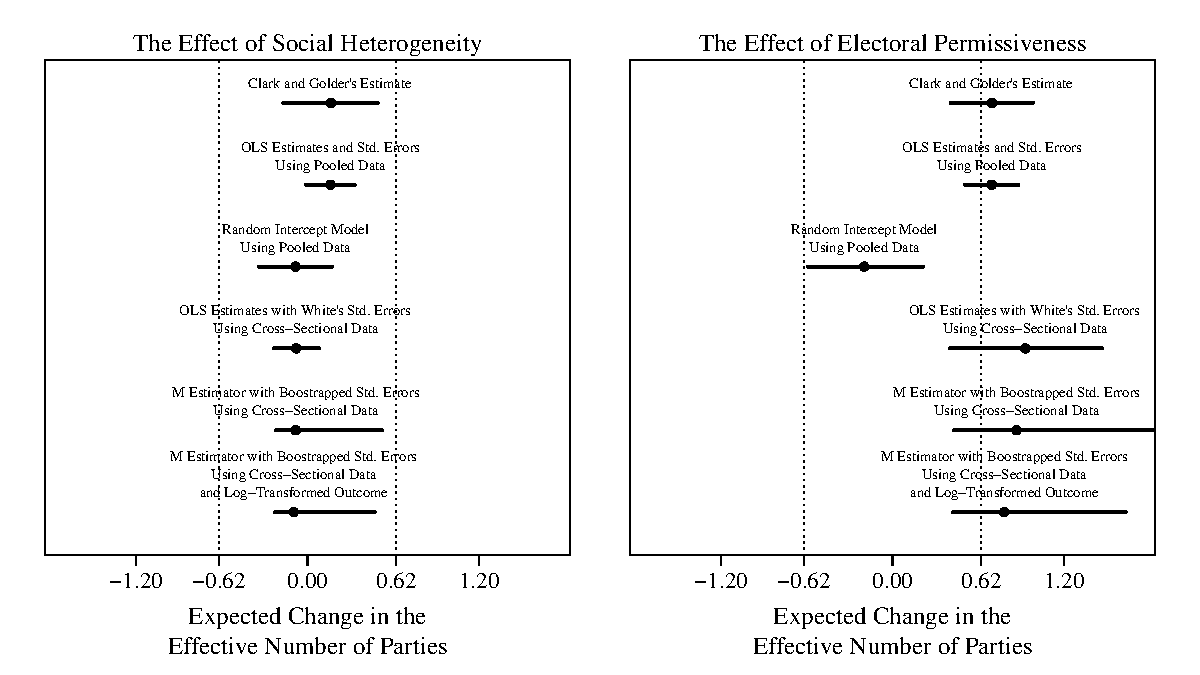
\includegraphics[scale = .7]{Figures/cg.pdf}
\caption{This figure shows the hypotheses based on the theoretical analysis of Clark and Golder (2006).
The hypotheses predict that the number of ethnic groups and the district magnitude should have a negligible effect on the number of political parties. I suggest in the text that any effect larger than 0.62 is substantively meaningful. Therefore the 90\% confidence intervals should fall in between the vertical dotted lines. The left panel shows that the data strongly suggest that social heterogeneity has only a negligible effect on the number of political parties when district magnitude is low, because the confidence intervals do not contain any meaningful effects. However, the right panel shows that the data do not support the conclusion that district magnitude has no meaningful effect when social heterogeneity is low. Of the six models I consider, only the confidence interval estimated by the random-effects model contains no meaningful effects.}\label{fig:cg}
\end{center}
\end{figure}

As \cite{ClarkGolder2006} show, the data support their hypotheses that (1) electoral permissiveness has a positive effect in heterogeneous societies and (2) social heterogeneity has a positive effect on the number of political parties when the electoral institutions are permissive.  However, Figure \ref{fig:cg} shows that the data offer mixed support for their hypotheses of negligible effects. 

When electoral institutions are constraining, social heterogeneity has no meaningful effect on the number of political parties. The left panel of Figure \ref{fig:cg} shows that the confidence intervals lie entirely within the region of substantively negligible effects. However, the right panel of  Figure \ref{fig:cg} shows no evidence for the hypothesis that electoral permissiveness should have a negligible effect on the number of political parties when the society is homogeneous. While the effect might be small, we cannot confidently reject meaningful effects (i.e., effects larger than 0.62), because they are consistently contained in the confidence intervals. Of the six models I consider, only the confidence interval estimated by the random-effects model contains no meaningful effects.

As Clark and Golder argue, but do not explicitly test, their data do suggest that increasing social heterogeneity has no meaningful effect on the number of political parties when electoral institutions are not permissive. While Clark and Golder show a small effect that is not statistically significant, the TOST offers a more compelling statistical test that rules out substantively meaningful effects. The data suggest that increasing the number of ethnic groups from 1.06 to 2.48 increases the number of parties  by about 0.5, at most. Thus, I find compelling evidence for Clark and Golder's claim that social heterogeneity has only  a substantively trivial effect under non-permissive electoral institutions.

While Clark and Golder make no explicit empirical claims about the effect of electoral institutions when social heterogeneity is low, their theoretical discussion suggests that when a society is homogeneous, electoral institutions should not lead to a substantively meaningful increase in the number of political parties. However, the data do not support this claim. I find that, even in one of the most socially homogeneous countries in the data set,  increasing district magnitude from one to seven might increase the expected number of political parties by more than one.  

\section*{Special Considerations for Researchers Arguing for Negligible Effects}

As with any statistical analysis, researchers arguing against meaningful effects must take deliberate steps to ensure they make valid and robust inferences. I conclude with several suggestions that might help applied researchers make more compelling arguments.

\textit{Design studies with interpretable effects.} The intersection-union approach requires special care in estimating interpretable effect sizes. In order to argue that an effect is not substantively meaningful, analysts cannot concern themselves only with the sign of the effects--the magnitude of the effects is crucial. Laboratory experiments, for example, require extra care in this regard. Treatments must be designed so that the size of their effects has a meaningful interpretation. For example, \citet[see also \citealt{Gerber2011}]{JeritBarabasClifford2013} explain that the magnitude of effects might vary across a laboratory and naturalistic setting. The most concerning possibility is that researchers design weak treatments that do not compare to natural, powerful treatments that occur outside the laboratory.\footnote{It is possible for researchers to design powerful treatments delivered in a pristine laboratory setting to attentive participants. These situations should generate larger treatment effects than comparable naturalistic settings \citep{Kinder2007}, biasing researchers away from finding support for hypotheses of no meaningful effect, but toward hypotheses of a positive or negative effect.} For example, a single negative campaign ad, though perhaps shown in a pristine lab environment, might not compare to a barrage of attack ads shown night after night during the evening news. Though such an experiment might have an immediate and brief impact on attitudes (e.g., \citealt{Ansolabehereetal1994}), it would be quite surprising if a single negative ad shown in a laboratory weeks before an election affected participants' actual political participation in a meaningful way. Treatments must be sufficiently powerful to generate a substantively meaningful effect if one exists.\footnote{\cite{ArceneauxNickerson2010} carefully argue, for example, that their ``null results'' are not due to a weak treatment. ``We recognize that a simple response to our findings is that our treatments were not `strong enough' to detect more arresting differential effects. Yet, we believe that three aspects of these studies minimize the persuasiveness of this critique. First, both campaigns remarked to us after the study that the negative messages were in some sense easier for volunteers to deliver, which, if anything, should have boosted their effectiveness...Finally, we do detect general message effects. Being exposed to either a positive or negative message did boost support for one of the propositions in Study 2.''}

\textit{Be mindful of measurement.} If concepts are poorly measured, a researcher might incorrectly conclude that a potential explanatory variable has only a negligible effect. For example, a researcher who codes any ad that mentions the other candidate as negative might find only a negligible effect on political participation. On the other hand, a researcher who codes an ad as negative only if it personally attacks the opponent might find a substantial demobilizing effect. Especially when arguing for negligible effects, it is crucial to clearly define theoretical concepts, identify any disjunction between concepts and their measures, and discuss the implications for the estimates and confidence intervals.

\textit{Carefully consider confounders.} Just as relationship between two variables can be spurious, so can a non-relationship. For example, suppose that while $X$ has a meaningful positive effect on $Y$, a third variable $Z$ has a positive effect on $X$ and a negative effect on $Y$. In this situation, $Z$ can disguise the meaningful relationship between $X$ and $Y$, leading the analyst to conclude that $X$ has no effect on $Y$ if $Z$ is not accounted for in the analysis. Standard methods, such as regression, should be used to account for potential confounders.

\textit{Use reliable data and perform many robustness checks.} No statistical method can overcome the problems associated with poor data and/or analysis. Just as empirical research is prone to biases when researchers expect positive or negative effects, it is prone to bias when researchers expect negligible effects. Reliable inferences require reliable data, good models of the data, and many robustness checks. Just as researchers hypothesizing a positive effect check that their conclusions are robust, so should researchers hypothesizing negligible effects. Each question and data set require different robustness checks, but analysts should be prepared to demonstrate that their results are robust to most plausible changes in the statistical technique.

Researchers often have theoretical expectations that explanatory variables should have only a negligible effect, at least in a particular context. However, these researchers are not restricted to using the absence of statistical significance as evidence for their claims. Instead, they can explicitly argue against meaningful effects by (1) using two one-sided tests to reject meaningful positive and meaningful negative effects or (2)
showing that the 90\% confidence interval contains only negligible values. This approach, combined with many robustness checks, enables analysts to make a compelling argument for a negligible effect.


%%%%%%%%%%%%%%%%%%%%%%%%%
%% References
%%%%%%%%%%%%%%%%%%%%%%%%%
\clearpage
\singlespace \normalsize
\bibliographystyle{apsr_fs}
\bibliography{bibliography}



\end{document}

